% !TeX root = ../main.tex
% Add the above to each chapter to make compiling the PDF easier in some editors.

\newtheorem{lemma}{Lemma}
\chapter{Monotonicity and Critical Payments}\label{chapter:monotonicity&criticalpayment}


To be a good solution for our proposed problem setting an approximation algorithm needs to be stragtegy proof. In order to prove this we are going to use the following Lemma by Blumrosen and Nisan \cite{BlNi07}, which we adapt to our setting in which the single minded players aren't buyers, but sellers.
\begin{lemma}
A mechanism for single-minded sellers in which losers get 0 is incentive compatible if and only if it satisfies the following two conditions:
\begin{enumerate}[label=\roman*)]
            \item \textbf{Monotonicity}: A seller who wins and sells at price $v_i^*$ keeps winning for any $v'_i<v_i^*$ (with the other sellers offers staying the same)
            \item \textbf{Critical Payment}: A seller who wins earns the maximum of all values $v'_i$ such that he still wins
\end{enumerate}
\end{lemma} 

\section{Monotonicity}

In order to prove that the Monotonicity criterium is fulfilled for our algorithm we need to guarantee for every Edge $e$, if $e$ is included in the output solution and we lower the cost of $e$ ($d(e)'=d(e)-\epsilon$ with $\epsilon > 0$) it stays included in the solution tree we obtain from running the algorithm again. To do this we are going to define $t$ as the approximated solution of the algorithm in question and $e, e'$ as two edges connecting the same nodes with cost $d(e)>d(e')$. With these definitions the monotonicity proof looks like this: 
\begin{proof}
$\forall e, e'$: $e\in t \implies e'\in t$
\end{proof}

\subsection{MST-Approximation}

To prove monotonicity for the MST-approximation we are going to walk through our implementation and check every step, where edge cost influences the algorithm and check what change a reduction in said cost could induce and whether this change could cause the solution to include different edges.
The point where edge cost affects the algorithm are:
\begin{enumerate}
\item creation of the metric closure using Floyd-Warshall 
\item creation of MST using Kruskal
\end{enumerate}
If both of these algorithm implement monotonicity we can safely deduce that the MST-approximation also implements Monotonicity.

Within the creation of the metric closure we used Floyd-Warshall's all-pairs-shortest-path algorithm, which checks for every triple of nodes $a,b,c$, whether the sum of the shortest paths $a\to b$ and $b\to c$ is less than the cost of the current shortest path $a\to c$ and updates it accordingly. Within every shortest path that includes $e$ and made it into the metric closure, the substitution of $e$ by $e'$ causes this path to be cheaper by $\epsilon$. Since every other shortest path will have its cost either unchanged or also reduced by $\epsilon$, if it also includes $e$/$e'$, there is no way for the shortest path to change in that case. Floyd-Warshall therefore implements for our case. It's possible for a shortest path that doesn't include $e$ to be replaced by a different one that includes $e'$, but this only improves the chances for $e'$ to appear in the solution tree.

The second point to look at is Kruskal's algorithm \cite{kruskal1956shortest}. Replacing the edge $e$ with $e'$ causes every edge that corresponds to a shortest path, which includes $e$ to be cheaper and therefore appear earlier in the sorted list. If $e$ was included in the output tree, than there aren't any cheaper edges in the metric closure, that connect the two components that $e$ connects. Since $d(e')<d(e)$ there can't be any cheaper edge than $e'$ either and therefore Kruskal's algorithm implements monotonicity and since Floyd-Warshall does so too we can conclude that the MST-approximation fulfills monotonicity.

\subsection{Berman-Ramaiyer}

For the algorithm by Berman and Ramaiyer we are going to procede like we did with MST and find the points, where the changed edge cost affects the algorithm.

The point where edge cost could potetially affects the algorithm are:
\begin{enumerate}
\item initialization of M to an MST-approximation
\item inclusion of $e$ in the remove-set
\item price of artificial edges in the add-set
\item MST-approximation of subsets $\tau$
\item replacement of remaining artificial edges in $N$
\end{enumerate}

We can quickly prove the first and fourth point since we already proved that the MST-approximation implements monotonicity. That means if the initial tree $M$ included $e$ it must include $e'$ and if it didn't then one of the $SMT(\tau)$ of subsets $\tau$ had to include $e$, since it has to be included in the final solution. If one of these trees $SMT(\tau)$ included $e$ it also has to include $e'$. Therefore the only thing we need to prove now is that the other three points at which the algorithm is affected don't lead to different subsets being included. 

Within the prepareChange a lot of changes might occur. Since the prepareChange splits the input tree at the maximum cost edge and adds this edge to the remove-set it's possible that $e$ could be included in a remove-set, while $e'$ isn't. But this only changes the fact, that now the cost of the remove-set may potentially assume any value within the range $d(R) \to d(R)-\epsilon$. Since $e$ ended up in the solution tree, the set originally either wasn't removed or $e$ was added in a subset tree $SMT(\tau)$. Therefore $e'$ not being in this remove-set doesn't change its inclusion into the solution tree. On top of the cost of the remove-set changing, there is also the changing cost of the artificial edge $f'$, that replaces $e'$ if $e'$ is part of the remove-set as well as the possibility of the $gain$ changing. The latter is especially crucial, since if the gain for a subset $\tau$ reaches zero the subset $\tau$ isn't considered in the construction phase anymore, which leads to $SMT(\tau)$ not being included in the solution. The $gain$ $g'$ of a particular subset $\tau$ can range after the replacement of $e$ by $e'$ from a minimum of $g-\epsilon$ to $g+\epsilon$ with $g$ being the $gain$ with unchanged edges. This is due to the scenario of the subset tree $SMT(\tau)$ not containing $e$, but containing $e'$. This would reduce the cost the tree and therefore increase $g'$ by $\epsilon$. The other scenario impacting $g'$ is with the remove-set computed by prepareChange including $e'$ and the $SMT(\tau)$ not. In this case the remove-set cost as well as the gain would be decreased by $\epsilon$. 
The important thing to note here is that, $g'-g$ is only negative, iff the subset tree $SMT(\tau)$ doesn't include $e'$, therefore the only inclusions that the algorithm may omit are the ones, that do not add $e'$ to the solution tree.  

The last point where the replacement of $e$ by $e'$ comes into play is in the construction phase, when the artificial edges of the add-sets are replaced by the minimal cost edge in $M$, that connects the created components. The fact that the minimal cost edge is the one that will be included makes it very easy to see that if $e$ was included here $e'$ will be too.

With all these critical points examined we can deduce that Berman and Ramaiyer's algorithm satisfies our monotonicity condition, which would make it a better choice than the MST-approximation, because of its better performance ratio. 
\subsection{Hougardy-Proemel}

For the $IRGH$ algorithm by Hougardy and Proemel, we are not going to try and prove it, instead we are going to show an example, where the monotonicity condition is violated. A fellow student at the Technical University of Munich has found a case, where the $RGH$ algorithm by Zelikovsky \cite{zelikovsky1996better} violates our monotonicity condition \cite{guggenbichler20}. If we use our $IRGH$ and choose $\vec{\alpha}=\{ 0\}$ we end up with 1 iteration of $RGH$ and the heuristic changes like this: 
$$f(B) = \frac{d(B) + \alpha * l(B)}{smt(T)-smt(T/B)} \Rightarrow f(B) = \frac{d(B)}{smt(T)-smt(T/B)}$$
Since the second heuristic is the one that is used in the $RGH$-implementation in question we can use this case to also violate monotonicity for the $IRGH$ by Hougardy and Proemel. Because it doesn't implement monotonicity this algorithm isn't strategy proof and therefore can't be reliably used for our problem setting. 

\section{Critical Payments}

After trying to prove monotonicity for all three algorithm we are going to compute critical payments for every edge in the solution tree. To find these critical payments we are going to use binary search. We are going to use the actual cost of the edge in question as our lower bound $L$ for the binary search and we are going to use exponential search to compute the upper bound $R$. 
To find this upper bound we double the cost of the edge in question $e$ and check whether it is still included in the solution tree. We repeat this process until it's not included anymore and we return this cost as our upper bound. With this upper bound we iteratively check whether $e$ is still part of the solution tree if we change its cost to $d(e)=m=\lfloor (L+R)/2\rfloor$. If it is then we put $L=m+1$ and otherwise we put $R=m$. Since we already know that $IRGH$ doesn't implement monotonicity and that the performance ratio of the MST-Approximation is inferior we are only going to compute the critical payments for the algorithm by Berman and Ramaiyer. The following figure \ref{fig:crit41} shows on the left the output of the Berman, Ramaiyer algorithm with unchanged edge costs and on the right it shows the same tree, but with every edge substituted by the critical payment cost of that edge. It is important to keep in mind, that each of these critical payments was computed with the rest of the tree unchanged, but since it would be unreasonable to print the same tree, with just one edge changed, once for every edge, i condensed it all into one tree. 

\begin{figure}[h]
\centering
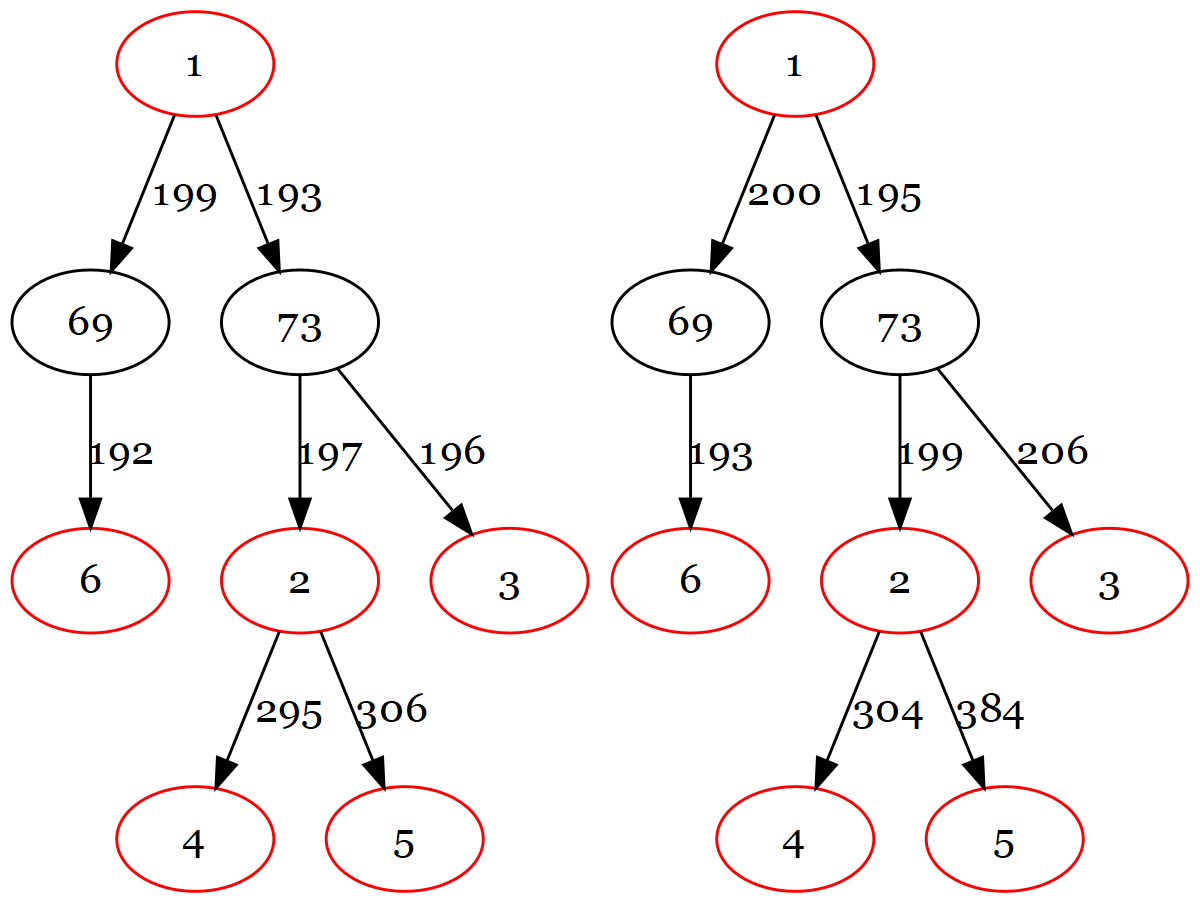
\includegraphics[scale=0.25]{figures/crit.png}
\caption{Output tree of testcase 41(left) and critical payments(right)}\label{fig:crit41}
\end{figure}
 
We can clearly see that most of these critical payments are just slightly higher, than the original cost. This is because there are a lot of other viable options in the graph we used, which was testcase 41. If there is an edge in the graph, that is irreplaceable e.g. if there is a terminal, that has a degree of one, within the graph, then its critical payment would be $\infty$, since it would always be included in the solution tree, no matter how high its cost. Now knowing the critical payments we can easily adjust our implementation of the Berman-Ramaiyer algorithm to always pay out the critical payment to the winning seller, which makes out algorithm implement critical payments. 


\section{Incentive Compatibility}

Using the Lemma by Blumrosen and Nisan \cite{BlNi07} we can conclude that MST-approximation algorithm as well as the algorithm by Berman and Ramaiyer are incentive compatible or strategy proof, if we modify it so that we always pay the critical payments to the winning seller, regardless of the price he offered us the edge for. Hougardy and Proemel's $IRGH$ algorithm doesn't implement monotonicity so we can use the aforementioned Lemma to disprove incentive compatibility for $IRGH$. Since we have proven strategy proofness for Berman, Ramaiyer's algorithm we can assume, that the valuations, that the sellers give us reflect their true valuations of the edges, that they are selling to us. 